\documentclass[11pt]{article}

\usepackage{graphicx} % for including graphics
\usepackage{amsmath} % useful maths macros, including \text
\usepackage{listings}
\usepackage{gensymb}
\usepackage{textcomp}
\usepackage{afterpage}
\usepackage{apacite}
\usepackage{acronym}
\usepackage{caption}
\usepackage{subcaption}

\usepackage{tikz}
\usetikzlibrary{shapes.geometric,arrows}
\tikzstyle{startstop} = [rectangle, rounded corners, text width=3cm,minimum width=3cm,
minimum height=1cm, text centered, draw=black, fill=red!30]
\tikzstyle{io} = [trapezium, trapezium left angle=70,trapezium right angle=110, minimum width=3cm, minimum height=1cm, text centered, draw=black, fill=blue!30]
\tikzstyle{process} = [rectangle, minimum width=3cm, text width=3cm,minimum height=1cm, text centered draw=black, fill=orange!30]
\tikzstyle{decision} = [diamond, minimum width=3cm, text width=3cm,minimum height=1cm, text centered, draw=black, fill=green!30]
\tikzstyle{arrow} = [thick,->,>=stealth]


\usepackage[bibstyle=ieee,citestyle=numeric-comp]{biblatex} % the cite style lets multiple refs in one bracket
\addbibresource{shared_resources/master.bib}



\renewcommand*{\multicitedelim}{\addcomma} % stops spaces between refs in single square bracket
% \usepackage{multicol}
% \usepackage{float}
\usepackage[a4paper, total={6.5in, 8in}]{geometry} % set the paper/text sizes
\def\apj{Astrophysical Journal}
\def\prd{Physical Review D}
\def\apjl{Astrophysical Journal Letters}



\title{\bf{Status and overview of deep-learning for gravitational wave parameter estimation}\\~\\
\large Submission of technical review paper}



\author{2259886}

\begin{document}
\maketitle

%%%%%%%%%%%%%%%%%%%%%%%%%%%%%%%%%%%%%%%%%%%%%%%%%%%%%%%%%%%%%%%%%%%%%%%%
%acronyms
%%%%%%%%%%%%%%%%%%%%%%%%%%%%%%%%%%%%%%%%%%%%%%%%%%%%%%%%%%%%%%%%%%%%%%%%

\acrodef{SNR}{signal-to-noise ratio}
\acrodef{LIGO}{Laser Interferometer Gravitational-wave Observatory}
\acrodef{MLP}{multi-layered perceptron}
\acrodef{cdf}{cumulative density functions}
\acrodef{pdf}{probability density function}
\acrodef{PE}{parameter estimation}
\acrodef{BBH}{Binary Black Hole}
\acrodef{BNS}{Binary Neutron Star}
\acrodef{VI}{variational inference}
\acrodef{CBC}{compact binary coalescence}
\acrodef{GW}{gravitational wave}

%%%%%%%%%%%%%%%%%%%%%%%%%%%%%%%%%%%%%%%%%%%%%%%%%%%%%%%%%%%%%%%%%%%%%%%%





\tableofcontents

\break
\section{Preamble}

Presented is a technical paper to account for the the status of my project in its first 5 weeks of research and preparation.

\subsection{Project overview}

Working within the UofG IGR-data group, my project is concerned with applying deep-learning methods to \ac{PE} of \ac{CBC} \ac{GW} signals. Specifically, working on an importance/rejection sampling feature to test the accuracy posterior distribution outputs from \texttt{VItamin\_b}~\cite{vitpaper}. Focusing on current \ac{BBH} signals, these results test \texttt{VItamin\_b}\textquotesingle s ability to handle future \ac{BNS} signals in preparation for low-latency multi-messenger astrophysics.

\subsection{Technical paper overview}

At such an early stage in my project research there are currently some significant holes in my knowledge which will be filled before my final report introduction is submitted. I have kept this paper as a hybrid between research-planning and presentation so it is in a far-from-polished layout. I have kept the section headings that I intend to include in my final report and will populate these with sufficient information as I continue my research.
\vspace{0.3cm}

\noindent
\textbf{Specific aspects missing from my knowledge:}
\begin{itemize}
  \item \ac{VI} methods (expecting a presentation within the IGR-data group week beginning 9th November, specifically Conditional Variational Autoencoders (CVAE)
  \item Better practical working knowledge of tensorflow~\cite{tensorflow}
  \item Specific template waveform banks used for \ac{PE} and the GR models used to create the waveforms across the parameter space
\end{itemize}

\noindent
\textbf{Report goals:}
\begin{itemize}
    \item 100 references (this seems to be a solid number to fit in with other publications of comparable generality/level of detail for an extended literature review introduction) 
    \item all figure text is large enough to be legible (got marked down for this last term)
    \item figure captions are stand-alone, of sufficient length and punctuation
    \item \ac{CBC} pipeline flowcharts (with deep-learning approaches sign-posted) formatted nicely as in Fig. 1 of Ref.~\cite{gstlal_gen1_2017}.
\end{itemize}



% \subsection{Word vomit}

% The properties of the sources can be inferred from theobserved gravitational waveforms.

% We are (in or beyond) the advanced-detector era, advanced = second gen detectors

% the advent of multimessenger astro in practise was gw170817 

% NIce phrasing: detector network of consitiuents....kagra, india lvc, (all ground-based)

% An international network of gravitational-wave (GW)detectors operating in the frequency band 10–103Hzexists today.

% The signal detection and interpretation is basedon a matched-filtering technique, where the noisy detec-tor output is cross-correlated with a bank of theoreticaltemplates.

% Motivation for PE: if we get accurate distance to event we can test hubble constant

% Adistinct advantageof the MCMC approach is that computational time does not grow exponentially withparameter number, as it does for other method

% The sky location of the source isprimarily determined through time of arrival differences atthe two Advanced LIGO sites. 

% Advanced ligo was upgraded before ther gw150914 hence the o1 and o2 ran on advanced ligo not initial ligo


% The amplitude of thesignal is maximum at the merger, after which it decaysrapidly as the final black hole rings down to equilibrium.

% most sensitive frequency band between 100 Hz and 300 Hz


% Note lower mass CBC systems have lower amplitude GW signals BUT HAVE MANY MORE orbits/cycles before merger so exist in sensitive LIGO band for longer hence better SNR

% o1 run, *advanced LIGO* min freq of bandwidth was only 30Hz, i believe its now only 20?

% state mass rnages for BH and NS etc

% o1 run limited search to binaries with combined mass (m1+m2 - not chirp mass) less than 100 solar masses, this is much diff now, yeh?

% nice population fig of o1 BBH template waveform bank from \cite{BBHo1} can I get an updated one for Mtot>100solar masses from gwtc2? would be nice comparison, could look in gwtc2 to see which bank(s) were used and see if the specific bank papers have nice figs? 

% % Things we want to improve:
% % \begin{itemize}
% %     \item speed (multi-messenger)
% %     \item sensitivity (higher bandwidth)
% %     \item computational cost (allow for higher data rate)
% %     % \item 
    
% \end{itemize}

\section{Origins and detections of \ac{GW} signals - focus on \ac{CBC} transients}

\begin{figure}[b!]
    \centering
    \includegraphics[width=.5\linewidth]{shared_resources/shared_figs/wos.png}
    \caption{Population of published works with keyword searches: \textit{Machine Learning} and \textit{Gravitational Waves}. A clear indication of increasing popularity of both fields essential for this work. Whilst the former search term has a factor of 10 greater popularity, both curves indicate rapidly evolving scientific fields. A clear increase in popularity of Gravitation Wave papers is seen after the 1st direct detection of a transient \ac{CBC} signal~\cite{abbott2016observation}. This is indicative of this seminal work accelerating the field into a new epoch of direct detections. Source \-- full-database search \textit{Web of Science, accessed November 2020}. }
    \label{fig:wos}
\end{figure}

% Talk about turn of the decade popularity. (mini abstract) *include key GW/GR equation(s)*

% Existing undetected as a mere speculation/hypothesis for 100 years their first detection a were five years ago, we find ourselves in an exciting time in the accelerating field of gravitational research. 

From their first hypothesis~\cite{einstein1} to the first direct detection of signal from binary black hole coalescence~\cite{abbott2016observation} by Advanced LIGO~\cite{advancedLIGO} and Advanced VIRGO~\cite{advacnedVIRGO} square-kilometre interferometers, we find ourselves in an exciting new epoch of gravitational physics. With the first two observing runs~\cite{BBHo1,gwtc1} and the first half of the third run~\cite{gwtc2} findings published along with corresponding public data release, the interest in gravitational waves is at an all time high (see figure~\ref{fig:wos}). 

As hypothesised in GR (insert citation - the same one as in theory section of~\cite{abbott2016observation}) gravitational waves are stretching/deformation of space-time from rotating massive objects. sources can be spilt into two types: continuous grav waves (CWs) and transient grav wave signals (GWs). Types of CWs are SN and ..?(2 citations at least) and much work has been done on these however in this work we are focused on the latter transient signals which are formed of GRBs(?) and CBCs.

The next section informs us how CBC signals are formed and how they are detected:

\subsection{Theoretical detection of \ac{CBC} \ac{GW} signals}

\begin{figure}[t!]
    \centering
    \includegraphics[width=.5\linewidth]{shared_resources/shared_figs/inspiral.png}
    \caption{Get good lengthy caption like in GW150914 observation paper.~\cite{abbott2016observation}}
    \label{fig:inspiral}
\end{figure}


Detection theory links straight from the brief intro of CBC grav wave origins, link to Fig.~\ref{fig:inspiral} HOW THE DETECTORS WORK....link to detector improvements in next subsection....Will talk here about Michelson interferometers and how the mirrors are used as test masses.


\subsection{Detector Network: Introduction and improvements}

\begin{figure}[t!]
     \centering
     \begin{subfigure}[t]{0.47\linewidth}
         \centering
         \includegraphics[width=\linewidth]{shared_resources/shared_figs/o2_asd.png}
     \end{subfigure}
     \begin{subfigure}[t]{0.47\linewidth}
         \centering
         \includegraphics[width=\linewidth]{shared_resources/shared_figs/o3a_asd.png}
     \end{subfigure}
    %  \vspace*{-7mm}
     \caption{Raw data acquired and recreated inspired by \cite{gwtc1,gwtc2} ASD show better sensitivity for advanced LIGO between o2 and o3 (thanks to the improvements made - link to paper) VIRGO is also much improved - use Joe's phd to talk about specific features of the ASD and how these have been improved between observations - then link to what improvements are currently being made prepping for o4 run, Joes phd: \cite{bayley2020phd}} 
     \label{fig:asd}
\end{figure}


Introduce the LVC detector network. The challenges they have faced for noise and how they have improved sensitivity in prep for o3 runs and how they are improving in prep for o4. (lots of refs of papers specific to practical improvements)

Future additions to network - KAGRA, INDIA etc. (need citations)

Having completed both o3 runs the detectors are currently undergoing improvements in prep for o4 run with more detectors added (mention more detectors being added). Previous improvements between 02 and 03 runs are BLANK [citation to direct improvements paper - there are loads - maybe cite 2-3 here)] focusing on ASD (see figure~\ref{fig:asd}). Will also use Joe's phd section as a good guide for recent improvements, specifically: actual features of the ASD plots and the processes that cause them.

As well as sensitivity, want to look at bandwidth as o1 run low-freq started at 30Hz~\cite{BBHo1}, report where it's at and that we are aiming for 10Hz. 

\subsection{Detection pipelines: Overview and Improvements}

\begin{figure}[t!]
    \centering
    \includegraphics[width=.6\linewidth]{shared_resources/shared_figs/number_events.png}
    \caption{Adapted from data release document LIGO-G1901322-v25, as presented in fig 1 of Ref.~\cite{gwtc2}. Stark increase in detection-rate comes from physical detector sensitivity improvements and pipelines being made more efficient.}
    \label{fig:events}
\end{figure}


Here is where I will have a quick rundown of the 2 search-pipelines PyCBC~\cite{pycbc2016} and GstLal (gen1 - \cite{gstlal_gen1_2017}, gen2 - \cite{gstlal_gen2_2019}) and their historical results/improvements throughout o1,2,3a runs.

In this section I want to include the first pipeline flowchart for detections (no deep-learning additions will be shown, instead deep-learning-enhancements for detection and PE pipelines will be shown in the  deep-learning section):

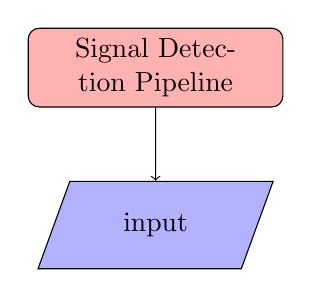
\begin{tikzpicture}[node distance=2cm][t!]
\node (start) [startstop] {Signal Detection Pipeline};
\node (label) [io, below of=start] {input};
\draw [->] (start) -- (label);
\end{tikzpicture}

End this section with the sky search pipelines being only half the story, link to PE pipeline which implements Bayesian methods: next section.

\section{Bayesian Inference for PE}

start this section with short intro of how important PE is, what motivates it (e.g. cosmo \-- estimate Hubble constant) 
and how it relies on Bayesian stats over frequentist MLE methods e.g. 

\subsection{Bayesian inference introduction}

NOTE - Bayesian itself is a general method of stats/prob whereas *Bayesian Inference* is the direct data analysis method of getting posterior prob from prior and likelihood.

Will do brief introduction of Bayes Theorem based on Sivia approach \cite{sivia2006textbook}


The below equations come from \cite{sivia2006textbook} and the original idea of bayes comes from the 18th century paper posthumously published \cite{bayesog}.

\begin{equation}
\label{eq:bayes_equal}
P(\theta|d) = P(\theta ) \frac{P( |\theta)}{P(d)}
\end{equation}

\begin{equation}
\label{eq:bayes_propto}
P(\theta|d) \propto P(\theta ){P(d |\theta)}
\end{equation}

\subsection{PE pipelines - Sampling methods, waveform models etc}

Will discus the improvements in PE pipelines between observing runs. Go into detail on different sampling methods (MCMC,NS and maybe into more niche ones like CPNest/Dynesty \-- with appropriate citations)

In this section will include the PE pipeline flowchart (again, no deep-learning in it yet):

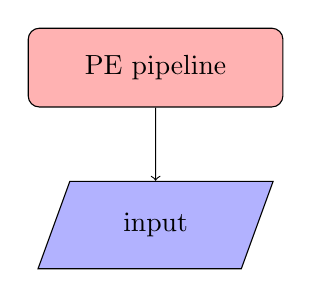
\begin{tikzpicture}[node distance=2cm][t!]
\node (start) [startstop] {PE pipeline};
\node (label) [io, below of=start] {input};
\draw [->] (start) -- (label);
\end{tikzpicture}

Note, end this section talking about with this increased detection-rate we find computing costs to be a real draw back. This motivates new approaches such as that from deep-learning, motivating the next section:


\section{Deep-Learning Approaches}


Start by mentioning the potential for deep-learning in the broad overall field of gravitational waves. Mention CWs and how deep-learning can be applied (Ref.~\cite{ml_cws}). Then specify down to transient CBC signals. Within this remit, discus the work done to implement deep-learning into the search pipeline (Ref.~\cite{gabbard2018matching}) (At this point I will create another flowchart for the Signal Detection pipeline which illustrates where deep-learning is applied) and then finally to PE pipeline (Ref.~\cite{vitpaper}) note, still not specifying BBH as we aim to expand Vitamin to handle BNS/NSBH signals.

Reiterate how it is a method to alleviate computer cost by a train-only-once method.

\subsection{General deep-learning introduction}

Give a brief insight into the underlying theory of deep-learning. Keep it broad but mention that PE is a regressional task and maybe then list a few different options of networks one could use for the PE problem. Then quickly take VI as our specific one and link to next section.

\subsection{Variational Inference and specifics of CVAE}

There is an upcoming talk on this week/beginning 9th November.

\subsection{\texttt{VItamin\_b}: How it works and improvements we want to make}

Discus Hunter's paper here.

Here, I would talk about how important low-latency is for multi-messenger applications then make new PE pipeline flowchart including the new VI methodology and including further multi-messenger pipeline attached.

\subsection{\texttt{VItamin\_b}: New feature \-- Importance sampling}

Use Australian paper~\cite{resample_aus} for a good guide for this intro section!
Go into the theory of how importance sampling works BUT dont go into specifics of what I specific did to implement it. That will go in the METHODOLOGY section following the INTRODUCTION in the final report!

\printbibliography[
heading=bibintoc,
title={References}
]



























































































\end{document}
